\section{Exercise 8}

Consider the stochastic process defined by the following diagram:
\begin{figure}[H]
    \centering
    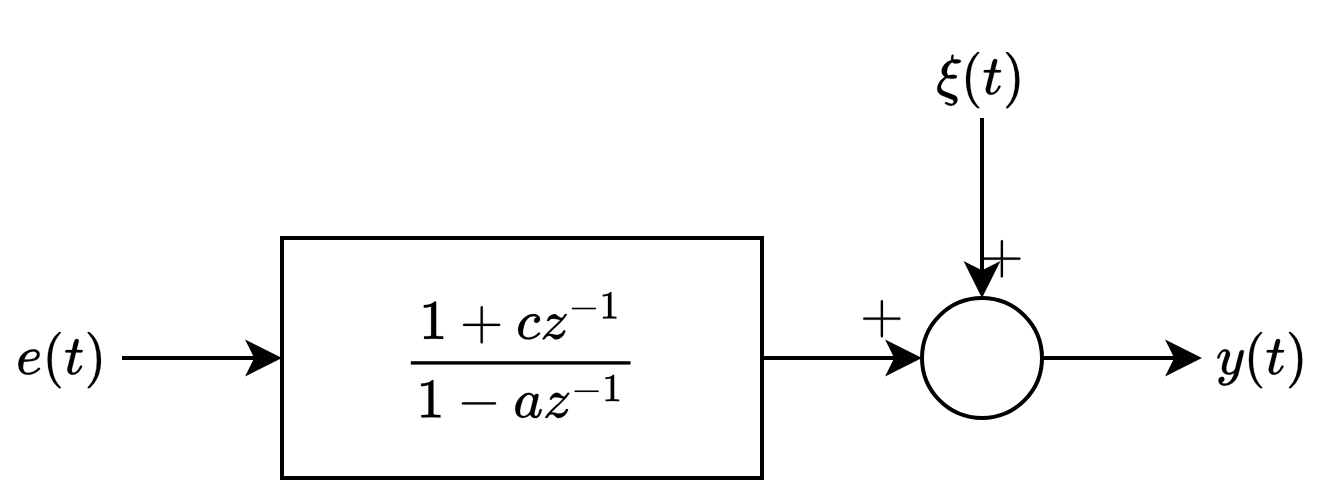
\includegraphics[width=0.5\linewidth]{images/block1.png}
\end{figure}
Here, $e(t) \sim WN(1,1)$ and $\xi(t) \sim WN(0,1)$ are uncorrelated.
\begin{enumerate}
    \item Determine when the process is stationary.
    \item Given $\gamma_y(0)=6$, $\gamma_y(1)=-2$, and $\gamma_y(\tau)=0$ for $\tau \geq 2$, compute the values of $a$ and $c$.
\end{enumerate}

\subsection*{Solution}
\begin{enumerate}
    \item The process $y(t)$ is stationary when both $\xi(t)$ and $y_1(t)$ are stationary.
        Since $\xi(t)$ is a  White Noise process, it is stationary by definition.
        The process $y_1(t)$ is stationary when $\left\lvert a \right\rvert<1$.
    \item Since $\gamma_y(\tau)=0$ for $\tau \geq 2$, this implies that $y(t)$ is a Moving Average Process of order one.
        Hence, $a=0$.

        The process in the time domain is: 
        \[y(t)=-ay(t-1)+e(t)+ce(t-1)+\xi(t)\]
        We can compute the covariance at $\tau=0$:
        \[\gamma_y(0)=\mathbb{E}\left[ {y(t)}^2 \right]=0\]
        From this, we obtain $c=\pm 2$. 
\end{enumerate}